\documentclass[UTF8,12pt]{ctexart}
\usepackage[a4paper,top=2cm,left=1.5cm,bottom=2cm,right=1.5cm]{geometry}
\usepackage[colorlinks,linkcolor=red,anchorcolor=green,citecolor=blue,urlcolor=cyan]{hyperref}
\usepackage{enumitem}
\usepackage{booktabs}
\usepackage{minted}
\newminted{cpp}{style=one-dark, autogobble}
\newmintinline{cpp}{style=one-dark}
\usepackage{tikz}
\usetikzlibrary{cd}
% title
\title{Qt大作业报告}
\author{赵陆森 2200013136, 潘聿阳 2200013219, 肖博文 2200013174}

\begin{document}
    \maketitle
    \tableofcontents
    \clearpage
    本说明文档采用\LaTeX 编写.
    \section{概述}
	    \subsection{代码结构}
	        本项目采用分文件编写的方式. 包括
	        \begin{table}[h]
	            \centering
	            \caption{界面头文件概述}
	            \begin{tabular}{cc}
	                \toprule
	                头文件                    & 功能概述                  \\
	                \midrule
	                \texttt{BattleField.h} & 包括一个战场类及其成员函数, 项目的基础  \\
	                \texttt{LevelChoose.h} & level mode选择关卡模式的实现   \\
	                \texttt{GameReview.h}  & survive mode战斗总结界面的实现 \\
	                \texttt{LevelReview.h} & level mode战斗总结界面的实现   \\
	                \texttt{Menu.h}        & 具体菜单部分的实现, 项目的核心      \\
	                \texttt{Ranking.h}     & 游戏排名界面的实现             \\
	                \texttt{Rule.h}        & 游戏规则界面的实现             \\
	                \bottomrule
	            \end{tabular}
	        \end{table}

	        \begin{table}[h]
	            \centering
	            \caption{内核头文件概述}
	            \begin{tabular}{cc}
	                \toprule
	                头文件                        & 功能概述           \\
	                \midrule
	                \texttt{\_Effect.h}        & 播放图片的效果基类      \\
	                \texttt{\_Entity.h}        & 飞机、子弹、道具等实体的基类 \\
	                \texttt{Bonus.h}           & 各种道具子类         \\
	                \texttt{Missile.h}         & 各种子弹子类         \\
	                \texttt{BackgroundMusic.h} & 背景音乐           \\
	                \texttt{Laser.h}           & 激光效果           \\
	                \texttt{ExplosionEffect.h} & 爆炸效果           \\
	                \texttt{TargetEffect.h}    & 瞄准效果           \\
	                \texttt{EnemyPlane.h}      & 各种敌机类          \\
	                \texttt{PlayerPlane.h}     & 玩家飞机类          \\
	                \texttt{BossEnemyPlane.h}  & Boss类          \\
	                \texttt{EnemyGenerator.h}  & 各种敌机生成策略类      \\
	                \texttt{Generator.h}       & 具体的关卡敌机生成设计    \\

	                \bottomrule
	            \end{tabular}
	        \end{table}

	        \begin{table}[h]
	            \centering
	            \caption{记录文件}
	            \begin{tabular}{cc}
	                \toprule
	                记录文件                     & 功能                     \\
	                \midrule
	                \texttt{DataRecord.txt}  & 记录survive mode中历史前五的得分 \\
	                \texttt{levelPRdata.txt} & 记录mode中玩家的表现得分         \\
	                \bottomrule
	            \end{tabular}
	        \end{table}

	        每个\texttt{.h}文件都有对应的\texttt{.cpp}文件实现\texttt{.h}文件中的函数,这将在后文详细描述.\par
	        此外, 本项目中图形化界面依赖于外部库\href{https://www.qt.io/zh-cn}{Qt}. 大部分界面使用图片作为背景.

	    \subsection{游戏结构}
	        整个游戏主要由四个界面组成: 开始界面, 模式选择界面, 战场界面, 战斗总结界面. 其中如果选择模式为\texttt{level mode}, 则会进入新的关卡选择界面. 战场界面为游戏核心.
	        游戏可选模式如下:
	        \begin{table}[h]
	            \centering
	            \caption{游戏模式}
	            \begin{tabular}{cc}
	                \toprule
	                模式                    & 简介                                 \\
	                \midrule
	                \texttt{survive mode} & 生存模式, 玩家生命值为0时游戏结束, 以冲击高分为目标       \\
	                \texttt{level mode}   & 关卡模式, 玩家可选择三种不同难度的关卡, 以打败最终Boss为目标 \\
	                \bottomrule
	            \end{tabular}
	        \end{table}
	        \begin{figure}[h]
	            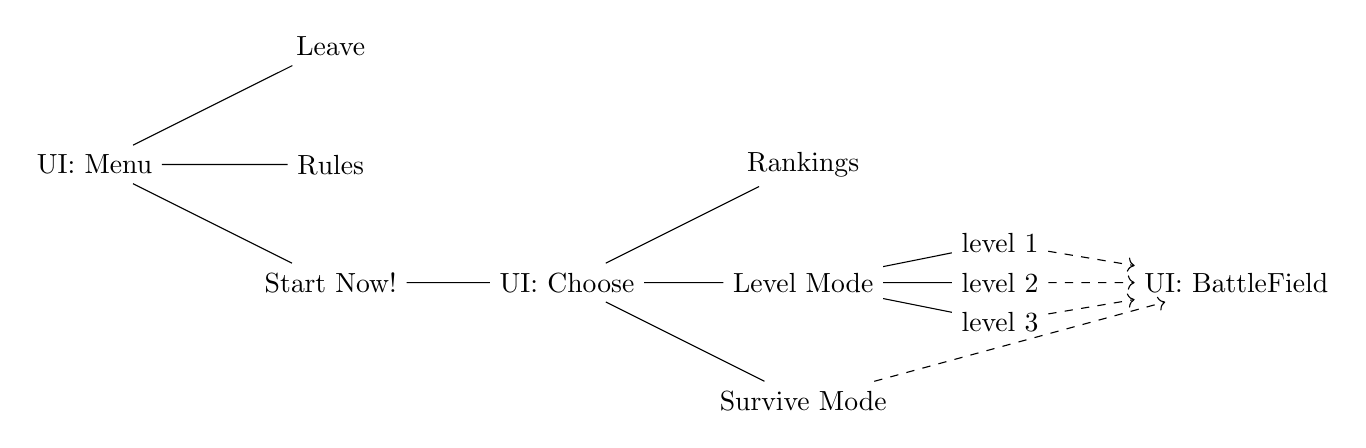
\begin{tikzpicture}
                    \node {UI: Menu}[level distance=30mm,grow=right]
                    child {
                        node {Start Now!}
                        child {
                            node {UI: Choose}
                            child { node (L0 node) {Survive Mode} }
                            child {
                                node {Level Mode}[level distance=25mm, sibling distance=5mm]
                                child { node (L3 node) {level 3} }
                                child {
                                    node (L2 node) {level 2}[level distance=30mm]
                                    child { node (BF node) {UI: BattleField} edge from parent[draw=none] }
                                }
                                child { node (L1 node) {level 1} }
                            }
                            child { node {Rankings} }
                        }
                    }
                    child { node {Rules} }
                    child { node {Leave} };
                    \draw[dashed,->] (L3 node) -- (BF node);
                    \draw[dashed,->] (L2 node) -- (BF node);
                    \draw[dashed,->] (L1 node) -- (BF node);
                    \draw[dashed,->] (L0 node) -- (BF node);

                \end{tikzpicture}
	        \end{figure}

	    \subsection{游戏主要功能}
	        \begin{enumerate}[nosep,label={\arabic*°: }]
	            \item 玩家:玩家通过\texttt{WSAD}操控飞机上下左右移动。\texttt{K}键释放一技能,射出一排子弹并清屏,单局限使用三次;\texttt{L}键释放二技能(有动画),清除沿路子弹,对敌机造成伤害,使用有冷却时间。\texttt{Esc}键暂停,\texttt{BackSpace}键退出本局游戏。
	            \item 敌机:敌机会发射子弹,子弹击中玩家或敌机与玩家碰撞均会造成伤害;敌机受玩家攻击若干次后会死亡,死亡后有概率掉落各种道具。
	            \item 道具。目前有如下道具:
	                \begin{itemize}[nosep]
	                    \item 加分道具:增加分数。
	                    \item 回血道具:恢复血量。
	                    \item 升级道具:升级子弹。升级次数有上限。
	                    \item 护盾道具:免疫一段时间内所有伤害。
	                \end{itemize}
	            \item Boss: Boss血量较高,目前有如下技能:
	                \begin{itemize}[nosep]
	                    \item 红色螺旋子弹
	                    \item 散开的星形子弹
	                    \item 黄色环形子弹
	                    \item 激光效果
	                    \item 网格形子弹
	                    \item 黄色追踪子弹
	                \end{itemize}
	            \item 背景音乐。
	            \item 数据存储,在外部的\texttt{.txt}文件中,游戏退出后也能保留。
	        \end{enumerate}

    \section{各文件内容描述}
	    \subsection{界面}
	        \subsubsection{\tt Menu.h, Menu.cpp}
	            \texttt{class Menu}, 完成所有界面相互切换的功能, 包括
	            \begin{enumerate}[nosep,label=\arabic*.]
	                \item 成员变量:
	                    \begin{itemize}[nosep]
	                        \item \texttt{vector<QPushButton*> startButtons}: 开始界面的按钮, 用来选择开始游戏, 离开游戏或者查看规则.
	                        \item \mintinline{c++}{vector<QLabel*> startLabels}: 按钮对应的图标, 用来标识现在鼠标指向的按钮.
	                        \item \mintinline{c++}{vector<QPushButton*> gameModes}: 模式选择界面的按钮, 用来选择\texttt{survive mode},\\
	                            \texttt{level mode}或者查看排行榜.
	                        \item \mintinline{c++}{vector<QLabel*> modeLabels}: 按钮对应的图标, 用来标识现在鼠标指向的按钮.
	                        \item \mintinline{c++}{vector<QWidget*> gameWidgets}: 用来储存所有的游戏界面, 方便切换.
	                        \item \mintinline{c++}{vector<QWidget*> to_remove}: 用来储存需要删除的界面, 最后在析构函数中一起删除.
	                        \item \mintinline{c++}{QLabel* Title}: 开始界面的标题
	                        \item \mintinline{c++}{QPushButton* toFirstPage}: 用来从关卡选择界面切换到开始界面.
	                        \item \mintinline{c++}{QStackedWidget* stackWidget}: \texttt{Qt}自带的控件, 这里用来在后端实现界面的切换功能.
	                        \item \mintinline{c++}{QVBoxLayout* menuButtonLayout, QHBoxLayout* mainLayout}: 用来控制界面控件的布局
	                    \end{itemize}
	                \item 函数:
	                    \begin{cppcode}
                        public :          
                            //槽函数
                            void StartGame();//切换到模式选择界面
                            void Leave();//结束程序
                            void ShowRules();//切换到游戏规则界面
                            void ToFirstPage();//切换到开始界面
                            void GameMode1();//切换到战场界面, 进入 survive mode
                            void GameMode2();//切换到战场界面, 进入 level mode
                            void GameMode3();//切换到游戏排名界面
                            void mouseMoveEvent(QMouseEvent* _event);//监听鼠标活动,在移动到按钮上时
                                                    // 触发颜色变换,图标显示等   
                    \end{cppcode}
	            \end{enumerate}
	            ~\par

	        \subsubsection{\tt GameReview, LevelReview}
	            这两个类都是用来进行游戏总结的, 除了界面的表观布局外实现的功能也基本一致. 其中界面的设计直接利用\texttt{Qt Designer}完成, 不再详细说明.
	            \begin{enumerate}
	                \item 成员变量
	                    \begin{itemize}
	                        \item \mintinline{c++}|int score|: 用来储存游戏得分, 进行表现星级评定.
	                        \item \mintinline{c++}|Menu* mainMenu|: 提供界面转换的接口, 在总结界面展示完后返回关卡选择界面.
	                    \end{itemize}
	                \item 函数
	                    \begin{cppcode}
                        void refill(); // 根据本次游戏成绩设置界面显示内容, 并更新记录文件
                        // 槽函数
                        void Return(); // 用来返回关卡选择界面
                    \end{cppcode}
	            \end{enumerate}
	        \subsubsection{\tt LevelChoose.h, LevelChoose.cpp}
	            这个类实现在\texttt{level mode}中选择关卡时的一系列效果, 为避免冗杂, 仅介绍关键变量和函数:
	            \begin{cppcode}
                //变量
                int PR_data[3];//记录从文件读取的历史表现评分, 与鼠标活动结合实现动态展示. 
                Menu* mainMenu;//提供界面转换的接口. 
                //槽函数
                void Level();//根据信号的触发者决定关卡编号, 并切换到对应的战场界面. 
                void mouseMoveEvent(QMouseEvent* _event);//监听鼠标活动
                void Return();//返回模式选择界面
            \end{cppcode}

	        \subsubsection{\tt Rule, Ranking}
	            \texttt{class Rule}完全由\texttt{Qt Designer}完成, 在\texttt{Qt}提供的\texttt{textBrowser}中导入\texttt{rule.md}来显示规则.

	            \texttt{class Ranking}实现\mintinline{c++}|void refill()|函数, 用来从\texttt{DataRecord.txt}中读取历史记录并展示.

	        \subsubsection{\tt BattleField.h}
	            \cppinline@BattleField@是游戏的核心。它继承自\cppinline@QWidget@类。
	            \begin{enumerate}[nosep,label={\arabic*. }]
	                \item 私有成员变量:
	                    \begin{cppcode}
                            QTimer* _timer; // 计时器
                            Ui::BattleFieldClass* ui; // Qt的UI界面
                            KeyState _key; // 按键记录
                            EnemyGenerator* _generator; // 关卡敌机生成,详见EnemyGenerator说明
                            Menu* mainMenu; // 主菜单
                        \end{cppcode}
	                \item 公有成员变量:
	                    \begin{cppcode}
                            QPixmap pic1, pic2; // 背景图片
                            std::vector<_EnemyPlane*> enemy_planes; // 存储当前全部敌机
                            std::vector<_Effect*> effects; // 存储当前需要展示的效果
                            std::vector<_Missile*> enemy_missiles; // 当前所有敌机子弹
                            std::vector<_Bonus*> drops; // 当前所有道具
                        \end{cppcode}
	                \item 成员函数
	                    \begin{cppcode}
                            BattleField(QWidget* parent = nullptr, Menu* menu = nullptr); // 构造函数
                            ~BattleField(); // 析构函数

                            void start(int level = 0); // 开始,参数指定关卡,会根据关卡编号修改_generator
                            void updateAll(); // 一帧内全部更新
                            void gameOver(); // 输掉游戏
                            void gameWin(); // 游戏胜利
                            void pause(); // 游戏暂停

                            // 以下函数在updateAll中调用
                            void generateEnemy(); // 生成敌机。调用_generator的函数
                            void checkDeadPlane(); // 清除死亡的敌机
                            void checkCollision(); // 碰撞检测
                            void paintEffect(QPainter& painter); // 绘制特效
                            void processKeyEvent(); // 处理按键
                            void updateMissiles(); // 更新子弹
                            void updateDrops(); // 更新掉落物
                            
                            void paintEvent(QPaintEvent* _event) final; // 重载绘制事件处理
                            void keyPressEvent(QKeyEvent* _event) final; // 重载按键按下事件处理
                            void keyReleaseEvent(QKeyEvent* _event) final; // 重载按键松开事件处理
                        \end{cppcode}
	            \end{enumerate}
	            \clearpage

	    \subsection{核心}
	        \begin{figure}[h]
	            \centering
	            \caption{核心代码结构}
	            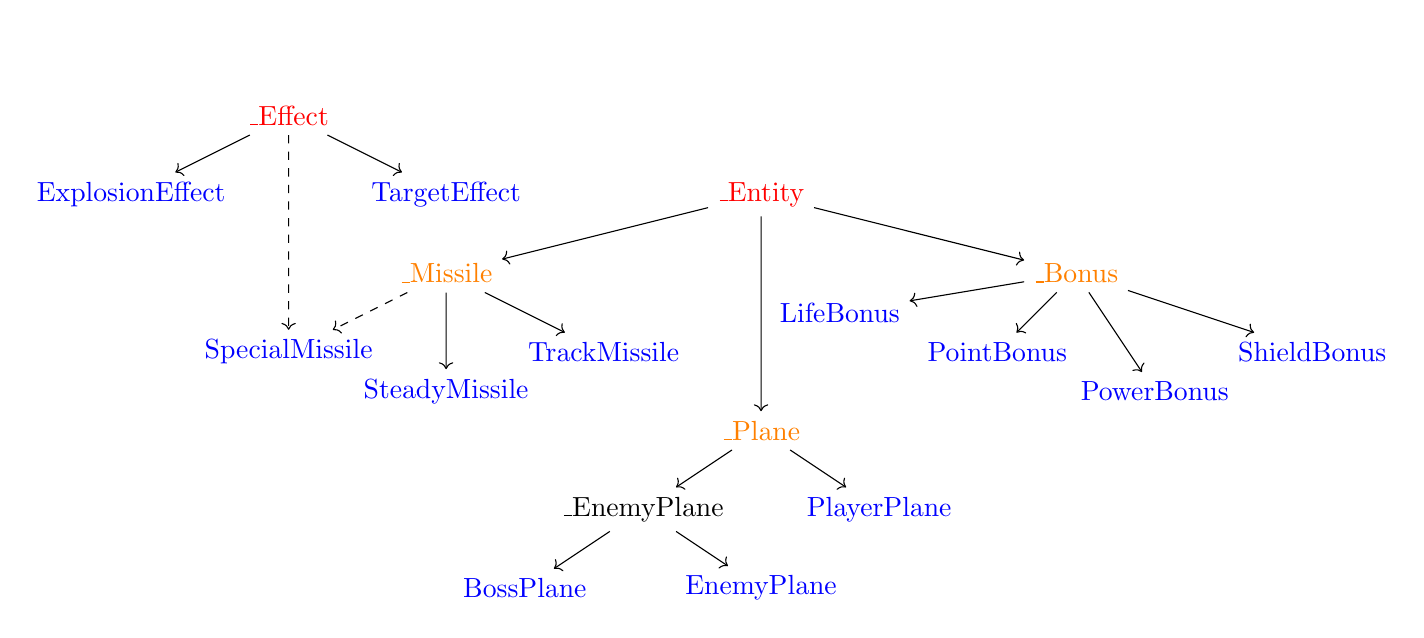
\begin{tikzpicture}
                    \node {}[sibling distance=60mm, level distance=10mm, ->]
                    child {
                        node[red] (Effect node) {\_Effect}[sibling distance=40mm]
                        edge from parent[draw=none]
                        child { node[blue] {ExplosionEffect} }
                        child { node[blue] {TargetEffect} }
                    }
                    child {
                        node[yshift=-10mm, red] {\_Entity}[sibling distance=40mm]
                        edge from parent[draw=none]
                        child {
                            node[orange] {\_Missile}[sibling distance=20mm]
                            child {
                                node[blue] (SpecialMissile node) {SpecialMissile}
                                edge from parent[dashed]
                            }
                            child { node[yshift=-5mm, blue] {SteadyMissile} }
                            child { node[blue] {TrackMissile} }
                        }
                        child {
                            node[yshift=-20mm, orange] {\_Plane}[sibling distance=30mm]
                            child {
                                node {\_EnemyPlane}
                                child { node[blue] {BossPlane} }
                                child { node[blue] {EnemyPlane} }
                            }
                            child { node[blue] {PlayerPlane} }
                        }
                        child {
                            node[orange] {\_Bonus}[sibling distance=20mm]
                            child { node[yshift=5mm, blue] {LifeBonus} }
                            child { node[blue] {PointBonus} }
                            child { node[yshift=-5mm, blue] {PowerBonus} }
                            child { node[blue] {ShieldBonus} }
                        }
                    };
                    \draw[dashed,->] (Effect node) -- (SpecialMissile node);
                \end{tikzpicture}
	        \end{figure}
	        上图箭头指示继承关系,红色为没有父类的基类,蓝色为没有子类的类

	        \subsubsection{\tt \_Effect.h}
	            类\cppinline@_Effect.h@, 用于显示图片。
	            \begin{enumerate}[nosep,label={\arabic*.}]
	                \item 成员变量:
	                    \begin{cppcode}
                            std::vector<QPixmap*> _pictures; // 存储要显示的图片
                            bool _valid; // 当前对象是否有效
                            int _picture_index; // 当前显示图片编号
                            int _timer; // 计数器
                        \end{cppcode}
	                \item 成员函数:
	                    \begin{cppcode}
                            _Effect(std::initializer_list<const char*> __images_path); // 构造函数
                            virtual ~_Effect(); // 析构函数
                            bool valid() const; // 返回_valid
                            virtual void update(); // 更新。默认情况增加计数器
                            virtual void display(QPainter& painter) = 0; // 要求子类实现绘制函数
                        \end{cppcode}
	            \end{enumerate}

	        \subsubsection{\tt \_Entity.h}
	            本文件包括:
	            \begin{itemize}[nosep]
	                \item 类\cppinline@_Entity@, 作为所有实体的基类。它包含成员变量
	                    \begin{cppcode}
                            QPixmap _picture; // 图片
                            QRectF _rect; // 矩形框,指示位置
                            bool _free = false; // 当前对象是否有效
                        \end{cppcode}
	                    并要求子类实现函数\cppinline|virtual void updatePosition() = 0;|用于一帧内位置更新。
	                \item 类\cppinline@_Plane@, 继承自\cppinline@_Entity@, 作为飞机的基类。它包含成员变量\cppinline@int _health;@表示飞机剩余血量。主要成员函数有:
	                    \begin{cppcode}
                            virtual void changeHealth(int m); // 飞机改变血量。虚函数是为了处理有护盾时受伤。
                            virtual void attack(_Plane* __other); // 攻击敌方飞机。判断是否相撞并改变血量。
                            virtual void drawOn(QPainter& painter); // 绘制飞机。
                        \end{cppcode}
	                \item 类\cppinline@_Missile@, 继承自\cppinline@_Entity@, 作为子弹的基类。它要求子类实现
	                    \begin{cppcode}
                            virtual void collide(_Plane* plane) = 0;
                        \end{cppcode}
	                    用于处理子弹与飞机的碰撞检测与更新。
	                \item 类\cppinline@_Bonus@, 继承自\cppinline@_Entity@, 作为道具的基类。它要求子类实现
	                    \begin{cppcode}
                            virtual void collide() = 0;
                        \end{cppcode}
	                    用于处理道具拾取与玩家状态更新。
	            \end{itemize}

	        \subsubsection{\tt PlayerPlane.h, EnemyPlane.h, BossPlane.h(Laser.h)}
	            这三个文件中的类均直接或间接继承自类\cppinline@_Plane@, 分别实现玩家飞机、普通敌机、Boss.

	            首先从\cppinline@_Plane@继承了子类\cppinline@_EnemyPlane@. 要求\cppinline@_EnemyPlane@子类实现
	            \begin{cppcode}
                    virtual void shootMissiles(BattleField* field) = 0;
                    virtual void afterDeath(BattleField* field) = 0;
                \end{cppcode}
	            然后从\cppinline@_EnemyPlane@派生出两个类\cppinline@EnemyPlane@(普通敌机)和\cppinline@BossPlane@(Boss).
	            \begin{enumerate}[nosep,label={\arabic*°: }]
	                \item 类\cppinline@EnemyPlane@有成员变量
	                    \begin{cppcode}
                            std::function<int(int)> _x, _y; // 横纵两方向的位置-时间函数
                            std::function<void(EnemyPlane*, BattleField*)> _shoot; // 发射子弹的函数
                            std::vector<double> _prob; // 掉落物的概率
                            int _shoot_timer = 0, _move_timer = 0, _shoot_interval; // 计时器
                        \end{cppcode}
	                    构造函数可以传入\cppinline@lambda@表达式,使用灵活。在命名空间\cppinline@Plane@下的\cppinline@Shoot@命名空间有常用的发射子弹的类(重载了小括号),\cppinline@Speed@命名空间有位置-时间函数的类(重载了小括号)。这些可以在构造函数中传入,避免重复的\cppinline@lambda@表达式。
	                \item 类\cppinline@BossPlane@中以各种技能为主,发射各种子弹。具体在功能部分有详细描述。\texttt{Laser.h}实现了其中激光技能的显示与判定。
	                \item 类\cppinline@PlayerPlane@继承自\cppinline@_Plane@, 是一个单例模式,即只有一个实例,无法在类外构造,只能通过\cppinline@PlayerPlane::plane()@获取。
	            \end{enumerate}

	        \subsubsection{\tt Bonus.h, Missile.h}
	            分别实现了多种道具类(继承自\cppinline@_Bonus@)和导弹类(继承自\cppinline@_Missile@)。具体在功能部分有详细描述。

	            值得一提的是特殊子弹类\cppinline@SpecialMissile@, 它继承自\cppinline@_Missile@和\cppinline@_Effect@两个类,让它具有子弹功能的同时可以播放一系列图片。

	        \subsubsection{\tt ExplosionEffect.h, TargetEffect.h}
	            均继承自类\cppinline@_Effect.h@, 分别实现敌机爆炸动画和导弹瞄准动画。

	        \subsubsection{\tt BackgroundMusic.h}
	            背景音乐。调用库\texttt{QtMultimedia}, 方便地进行音乐播放、暂停、切换。

	        \subsubsection{\tt EnemyGenerator.h, Generator.h}
	            这两个文件对敌机生成进行进一步整合。

	            \texttt{EnemyGenerator.h}中主要实现类\cppinline@EnemyGenerator@. 它作为\cppinline@Battlefield@的成员,规定了一次游戏全程的生成策略。一个\cppinline@EnemyGenerator@包含多个\cppinline@Policy@, 它们顺序执行,构成一个完整关卡。一个\cppinline@Policy@代表一阶段的生成策略。\cppinline@Policy@有多个子类:
	            \begin{itemize}[nosep]
	                \item \cppinline@EnemyGeneratingPolicy@: 当前生成普通敌机。类含有一个由一列函数对组成的成员,函数对中前者指明生成什么敌机,后者指明何时生成敌机。
	                    \begin{cppcode}
                            typedef std::function<EnemyPlane*()> plane_t;
                            typedef std::function<bool()> flag_t;
                            std::vector<std::pair<plane_t, flag_t>> _policy;
                        \end{cppcode}
	                    计时结束后进入下一阶段。
	                \item \cppinline@BossGeneratingPolicy@: 当前出现Boss. 直到Boss死亡才进入下一阶段。
	                \item \cppinline@EnemyClearingPolicy@: 这段会让场上所有普通飞机强制向前移动直到全部消失,一般为下面Boss出现做准备。
	                \item \cppinline@PictureDisplay@: 这阶段会展示图片一段时间。
	                \item \cppinline@MessageDisplay@: 这阶段会展示文字一段时间。
	            \end{itemize}
	            \vspace*{0.5\baselineskip}\par
	            \texttt{Generator.h}中为每局游戏指定阶段流程。其中无尽模式会循环,关卡模式在所有阶段结束后会结算。

    \section{小组分工}
	    \begin{table}[h]
	        \centering
	        \begin{tabular}{cc}
	            \toprule
	            组员      & 分工                       \\
	            \midrule
	            赵陆森(组长) & 游戏主体部分代码框架搭建,参与设计游戏关卡及功能 \\
	            潘聿阳     & 设计游戏关卡及功能,参与游戏主体部分代码框架搭建 \\
	            肖博文     & 游戏界面逻辑实现,包括积分系统等         \\
	            \bottomrule
	        \end{tabular}
	    \end{table}

    \section{项目总结与反思}
	    本次程序设计大作业是我们第一次以小组合作的形式完成一个项目,也是第一次使用\texttt{Qt}这一\texttt{C++}库。从这个项目我们学到了很多知识。

	    首先,小组合作的形式要求我们的代码必须有良好的命名规范。同时我们也要保持良好的代码结构,进行分文件编写,将不同组员实现的部分——界面和游戏核心通过\cppinline@BattleField@类的几个函数相联系。

	    其次,项目在编写过程中可能会不断有新功能加入,因此编写时要注意类编写时的可拓展性,如\cppinline@EnemyPlane@类传入\cppinline@lambda@表达式作为参数。为了关卡编写方便起见,我们把一个关卡的流程(显示文字信息、普通敌机、Boss)的阶段抽象成类\cppinline@Policy@的子类,类\cppinline@EnemyGenerator@则有一系列阶段组成,便于关卡设计实现。

	    我们在这一过程中也学习了\texttt{Qt}库的使用,熟悉了\texttt{Qt}库的\texttt{.ui}文件的可视化编辑,了解了\texttt{Qt}库信号与槽的机制,掌握了对一部分\texttt{Qt}内置类的使用或继承。

	    此外,开发过程中我们使用\texttt{git}进行版本控制和同步,了解了\texttt{github}基本使用方式。

\end{document}
